\FloatBarrier
In Teilchendetektoren finden folgende Wechselwirkungen von Photonen mit Materie statt:

\begin{figure}[H]
	\centering
	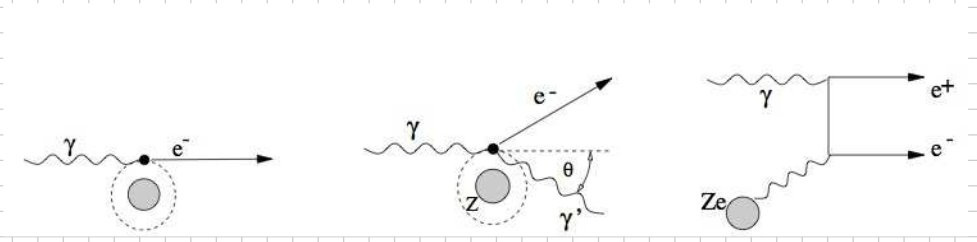
\includegraphics[width=\textwidth]{1-wewiMitMaterie.jpg}
\end{figure}

Bei niedrigen Energien überwiegt der Photoeffekt, bei dem das Photon seine gesamte Energie auf ein
Hüllenelektron überträgt. Bei mittleren Energien kommt der Compton-Effekt hinzu, der eine elastische
Streuung eines Photons an einem Hüllenelektron beschreibt. Bei hohen Energien überwiegt schließlich
die Paarbildung, bei der ein Photon im Kernfeld in ein $e^+e^-$-Paar konvertiert.

\begin{figure}
	\centering
	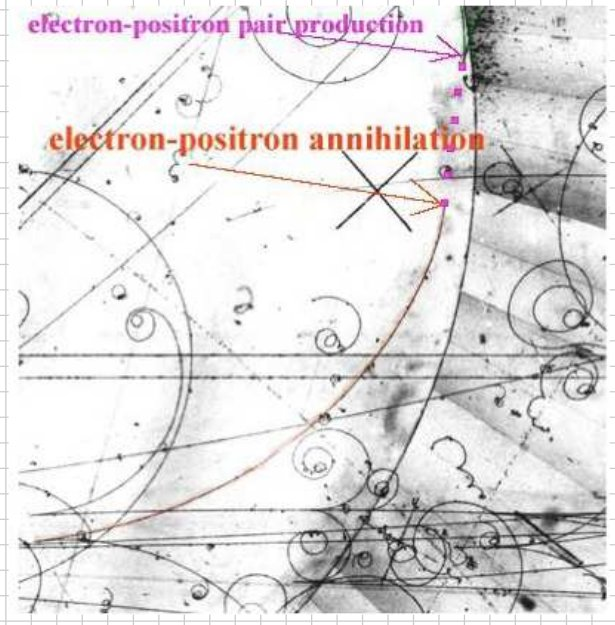
\includegraphics[width=0.5\textwidth]{2-pairProduction.jpg}
\end{figure}

Bei sehr niedrigen Photonenergien kommt es zur Thomson- und Rayleighstreuung (s. Kap.
\ref{thomsonrayleigh}).
\\
Für Photonen relevante Energiebereiche sind  

\begin{itemize}
  \item UV-Licht: eV
  \item Röntgenstrahlung: eV-keV
  \item Gammastrahlung: keV-MeV
\end{itemize}

Ein wichtiger Unterschied zu geladenen Teilchen besteht darin, dass die obigen Prozesse einzelne
Photonen streuen bzw. absorbieren und diese dadurch aus dem Strahl entfernt werden. Die Energie der
Photonen bleibt unverändert (Ausnahme: Compton-Effekt), es kommt nur zu einer Verringerung der
Intensität.

\FloatBarrier
\subsubsection*{Quantitative Beschreibung}

Photonen werden mit einer Wahrscheinlichkeit, die proportional zur Wegstrecke $\mathrm{d}x$ ist,
absorbiert bzw. beim Compton-Effekt gestreut. Wir definieren einen Absorptionskoeffizienten $\mu$,
der die Absorptionswahrscheinlichkeit pro Wegstrecke angibt:

\[ -\frac{1}{N}\cdot\frac{\mathrm{d}N}{\mathrm{d}x}=\mu.\]

Mit der Anzahl $\mathrm{d}N_T$ der Targetteilchen pro Strecke $\mathrm{d}x$ und Fläche $F$ (also
dem Volumen $V$), dem Atomgewicht $A$, der Teilchendichte $n$ und dem Absorptionswirkungsquerschnitt
$\sigma$ erhält man

\[N_T=\frac{\rho\cdot V}{A}\cdot N_A\]
\[\Rightarrow~~~n=\frac{N_T}{V}=\frac{\rho}{A}\cdot N_A\]
\[\Rightarrow~~~-\frac{1}{N}\frac{\mathrm{d}N}{\mathrm{d}x}=\mu=\frac{\mathrm{d}N_T}{\mathrm{d}x}\cdot
\frac{\sigma}{F}=\rho\cdot\frac{N_A}{A}\cdot\sigma=n\cdot\sigma \]

Die mittlere freie Weglänge $\lambda$ ist

\[ \lambda = \frac{1}{\mu}=\frac{1}{n\cdot \sigma} \]

Auch hier sind die auf die Dichte 1 bezogenen Größen in der Literatur zu finden
(Massenabsorptionskoeffizienten). 
\\
Es gilt

\[ \frac{\mu}{\rho}=\frac{N_A}{A}\cdot \sigma \]

\begin{figure}[H]
		\centering
		\includesvg[svgpath=bilder/1-1/]{photonen}
\end{figure}

Die Anzahl der Photonen im Strahl folgt dem Exponentialgesetz

\[N(x)=N_0\cdot e^{-\mu x} \]

\begin{figure}[H]
	\centering
	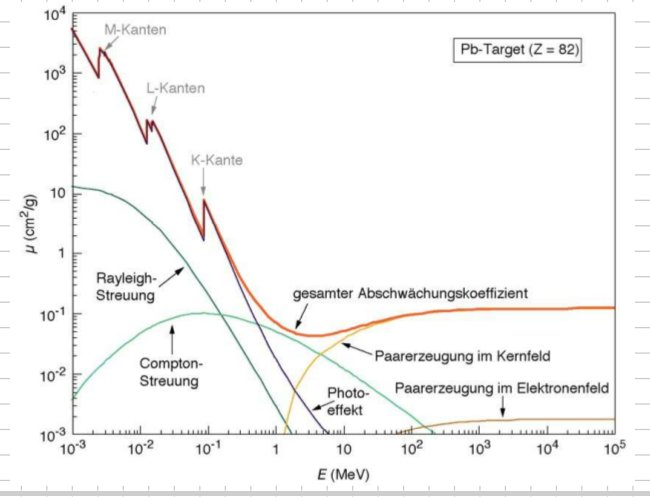
\includegraphics[width=0.5\textwidth]{3-alleEffekte.jpg}
\end{figure}

Abgesehen von einem engen Bereich um etwa $1\,$MeV dominieren Paarbildung und Photoeffekt. Die
Prozesse finden in Abhängigkeit der Energie, aber auch der Kernladungszahl $Z$ des Targets statt. 

\begin{figure}[H]
	\centering
	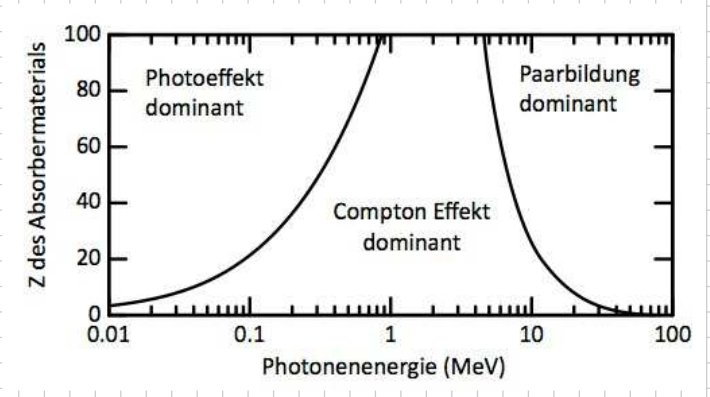
\includegraphics[width=0.5\textwidth]{4-effekteInAbhaengEnergie.jpg}
\end{figure}

Die Abhängigkeiten werden in den folgenden Kapiteln diskutiert. 
\FloatBarrier